\documentclass[11pt, a4paper]{article}
\usepackage{graphicx} 
\usepackage[left=1in, right=1.65in, top=1in, bottom=1in, margin=1in]{geometry}
\setlength{\parindent}{2em}
\newcommand{\miparrafo}[1]{\hspace{1.5em} #1\par}
\usepackage{caption}
\usepackage{setspace}
\setstretch{1.2}
\usepackage{float}
\usepackage{amsmath}
\usepackage[colorlinks=true, linkcolor=blue, urlcolor=blue]{hyperref}
\usepackage{array}
\usepackage{longtable}
\usepackage{tabularx}
\usepackage{enumitem}
\usepackage[utf8]{inputenc}
\usepackage[normalem]{ulem}
\usepackage{xcolor}
\usepackage{siunitx}
\usepackage{booktabs}
\usepackage{dcolumn}
\usepackage{placeins} 
\usepackage{threeparttable}
\usepackage{fancyhdr}
\usepackage{multirow} 
\usepackage{adjustbox}
\usepackage{makecell}
\usepackage{hyperref}



\fancyhead[L]{\textbf{Machine Learning}}
\fancyhead[R]{\textbf{Maestría en Economía}}
\setlength{\headwidth}{\dimexpr\textwidth+\marginparsep}

\geometry{
    top=1in,
    bottom=1in,
    left=1in,
    right=0.86in,
    % Otras opciones de tamaño de página...
}

\begin{document}

\begin{titlepage}
    \centering
    \vspace*{2cm}
    {\huge\bfseries Machine Learning  \par}
    \vspace{0.5cm}

    {\huge\bfseries Problem Set 01  \par}
    \vspace{0.5cm}
    \vspace{0.5cm}
    {\huge\bfseries\par}
    \vspace{3cm}
    
    {\Large \textbf{Gómez Dalila y Camilletti Celina} \par}
    {\large Maestría en Economía \par}
    {\large Universidad Nacional de La Plata}
    \vspace{1cm}
  
  \begin{figure}[H]
    \centering
    \captionsetup{justification=centering}
    
\includegraphics[width=5cm]{../Views/UNLP_Logo_(cropped).svg.png}
\end{figure}
\end{titlepage}


\section{Introducción}
La estimación de los ingresos laborales es de gran relevancia en el ámbito económico, ya que permite comprender las dinámicas del mercado laboral y las desigualdades en la distribución de la riqueza. No obstante, un análisis preciso de los ingresos va más allá de la dimensión económica; en el sector público, la correcta declaración de los ingresos individuales es esencial para el cálculo de impuestos. Sin embargo, el fraude fiscal derivado de la subdeclaración de ingresos ha sido un problema significativo y persistente. En este contexto, un modelo de predicción de ingresos puede ser útil no solo para identificar casos de fraude y reducir la brecha entre lo que debería recaudarse y lo efectivamente recaudado, sino también para identificar a individuos y familias vulnerables que requieran asistencia adicional.

El presente trabajo se centra en la predicción del salario horario utilizando una muestra de datos de la Gran Encuesta Integrada de Hogares (GEIH) realizada en Bogotá en 2018 por el Departamento Administrativo Nacional de Estadística (DANE), bajo el título "Medición de Pobreza Monetaria y Desigualdad Report". Esta encuesta tiene como objetivo proporcionar información estadística sobre el mercado laboral, los ingresos, la pobreza monetaria y las características sociodemográficas de la población residente en Colombia.

Todas las estimaciones computacionales realizadas en el presente trabajo se encuentran debidamente presentadas en el \href{https://github.com/Dalila02/ML_PS01}{repositorio ML-PS01} creado por las autoras.

El objetivo principal de este trabajo es obtener la mejor predicción del salario horario utilizando modelos lineales y técnicas de remuestreo, como el \textit{Validation Set Approach} y el \textit{Leave-one-out cross-validation (LOOCV)}. Estas técnicas de remuestreo permiten evaluar los modelos de predicción sobre datos de prueba o fuera de muestra, basándose en los modelos creados con los datos de entrenamiento. Esto se realiza porque los modelos pueden ajustarse excesivamente a los datos de entrenamiento, lo que los haría ineficaces si se aplicaran a nuevas observaciones o para realizar predicciones futuras, que es el propósito final de los modelos.

Los resultados preliminares sugieren que factores como la edad, el nivel educativo, la formalidad del empleo y el tamaño de la empresa son determinantes clave para la predicción del salario horario.

\section{Datos}

Este análisis utiliza una muestra de datos tomados de La Gran Encuesta Integrada de Hogares (GEIH)  realizada en Bogotá en el año 2018 por el Departamento Administrativo Nacional de Estadística (DANE) , la cual se denomina \textit{"Medición de Pobreza Monetaria y Desigualdad Report"},para predecir el ingreso empleando una variedad de características que capturan aspectos personales. 

 La GEIH tiene como objetivo proveer información estadística relacionada con mercado laboral, ingresos y pobreza monetaria, así como de las características sociodemográficas de la población residente en Colombia.  Se trata de una encuesta continua, que se aplica en todo el territorio nacional y que permite la desagregación de resultados para el total nacional, total cabeceras, total centros poblados y rural disperso, con un alcance mensual de aproximadamente 25.000 hogares , lo cual permite obtener una amplia variedad de información de cada encuestado y su hogar.  

Los datos utilizados fueron obtenidos mediante scraping, totalizando 32.117 observaciones y 177 variables, que capturan diversas características individuales en categorías como trabajo, ingresos, educación, situación de pobreza, residencia ,estado de discapacidad, relaciones familiares, beneficios sociales,etc.  La alta dimensionalidad es adecuada para las técnicas de aprendizaje automático, ya que muchos de los modelos pueden manejar eficazmente esta característica a través de la selección de variables y otras técnicas.

No obstante, para el análisis se incluyeron únicamente individuos empleados mayores de dieciocho (18) años que contaron con ingresos reales positivos y no nulos, de manera que se pudiera calcular el logaritmo natural de la variable, con el objetivo de normalizar los datos y aumentar la interpretabilidad de las métricas de evaluación. Asimismo, se eliminaron las observaciones con valores missing de la variable \textit{"maxEducLevel"}, la cual captura el máximo nivel educativo alcanzado por los trabajadores. Como resultado, la muestra se redujo a 9784 observaciones. 
 
La Tabla 1 describe las principales estadísticas descriptivas del logaritmo del salario horario y de posibles variables relevantes para la explicación del mismo. Las variables \textit{Sexo}, \textit{Formal} y \textit{College} son variables dicotómicas que toman valor unitario en caso de que el individuo sea hombre, con empleo formal y educación terciaria finalizada, y cero en caso contrario.

\begin{table}[ht]
    \centering
    \caption*{\textbf{Resumen de estadísticas descriptivas}}
    \begin{adjustbox}{max width=\textwidth}
        \begin{tabular}{lcccccccc}
            \toprule
            & \textbf{Observaciones} & \textbf{Media} & \textbf{Desvío Estándar} & \textbf{Mínimo} & \textbf{25\%} & \textbf{50\%} & \textbf{75\%} & \textbf{Máximo} \\
            \midrule
            Salario horario        & 9784 & 8.7309 & 0.7263 & 5.7889 & 8.3491 & 0.5315 & 8.9998 & 12.7674 \\
            Edad                       & 9784 & 36.4384  & 11.937 & 19  & 27   & 34   & 45   & 86     \\
            Sexo                       & 9784 & 0.5017  & 0.5000 & 0   & 0    & 1    & 1    & 1      \\
            Formal                   & 9784 & 0.7728   & 0.4190 & 0   & 1    & 1    & 1    & 1      \\
            College                  & 9784 &  0.3440   &  0.4751 & 0   & 0 & 0    & 1    & 1      \\
            \bottomrule
        \end{tabular}
    \end{adjustbox}
\end{table}

 En la muestra de referencia, el salario horario promedio de la economía colombiana para el año 2018 fue de \$6.191,30 con un valor máximo de \$326,67 y máximo de \$35.0583,43. A su vez, el 50\% de los trabajadores ocupados tienen 27 años de edad o menos, mientras que, la edad promedio es de 36 años, lo cual vislumbra el sesgo generado por aquellos trabajadores con edades superiores (máximo 86 años) que tienden a elevar la edad promedio. 
Finalmente, al analizar la estructura poblacional de los trabajadores ocupados se observa que el 50.17\% son hombres, 77.28\% se encuentran bajo un trabajo formal y el 34.40\% cuentan con terciario completo. 

La Figura 1 describe las funciones de densidad del salario laboral horario para distintos grupos de referencia; i) Formales vs Informales, ii) Hombres vs Mujeres y iii) Universitarios vs No Universitarios. 

\begin{figure}[H]
    \centering
	\caption*{\textbf{Figura 1. Funciones de Densidad del Salario Laboral Horario por grupos de interés}}
  	\captionsetup{justification=centering}
  	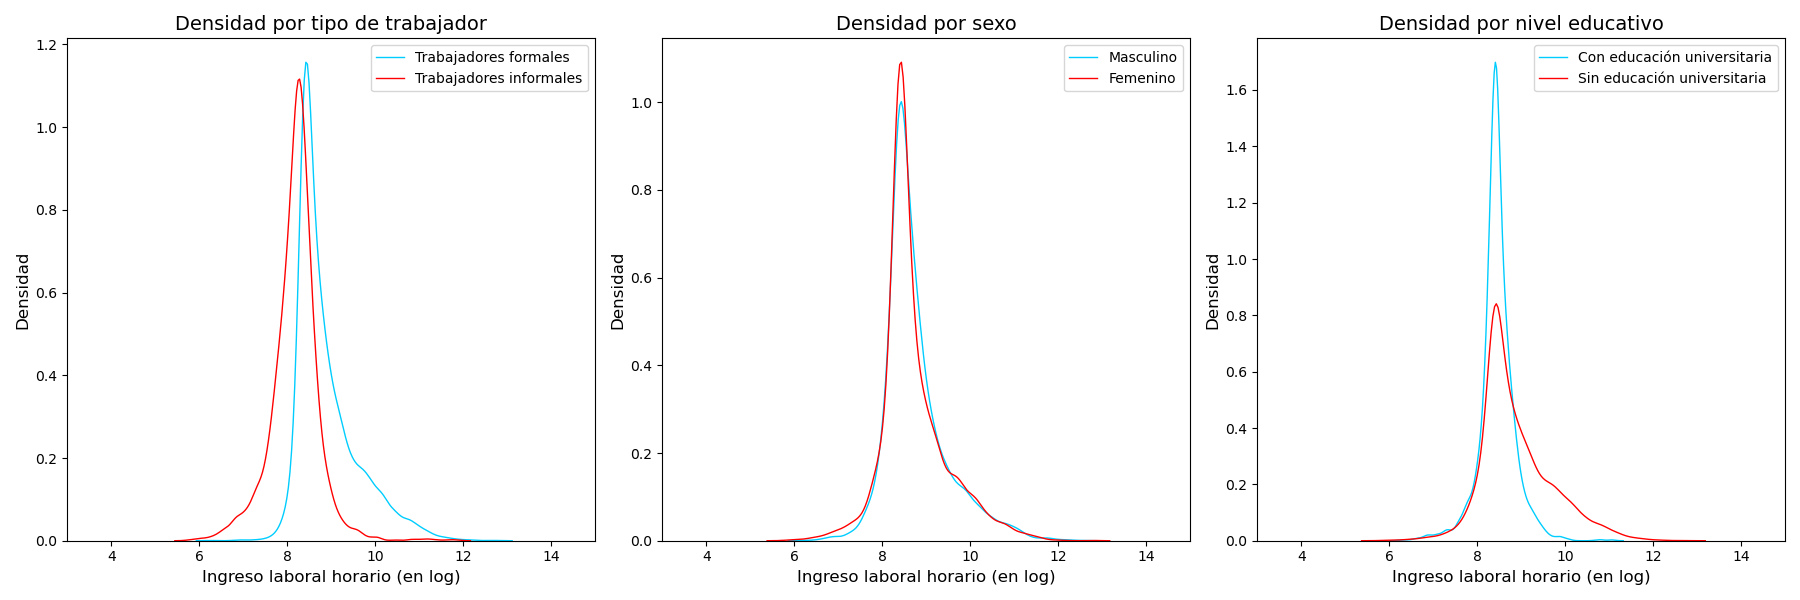
\includegraphics[width=16cm]{../Views/grafico1.png}
	\caption*{\small Fuente: Elaboración propia con base en datos de la GEIH }
\end{figure}

Se observa que, en promedio, el salario laboral por hora es más alto entre los trabajadores formales que entre los informales. Asimismo, la proporción de mujeres con un ingreso promedio supera a la de los hombres, y esta tendencia se repite al comparar individuos con educación universitaria frente a aquellos que no la poseen, contando estos últimos con uns dispersión de ingesos superior. 

Finalmente, con el objetivo de predecir la variable objetivo, el ingreso laboral nominal por hora de los asalariados, la Figura 2 presenta una matriz de correlación que incluye las principales variables de la muestra que, conforme la literatura económica, podrían ser relevantes para pronosticar dicha variable. 

\begin{figure}[H]
    \centering
	\caption*{\textbf{Figura 2. Matriz de correlaciones}}
	\captionsetup{justification=centering}
	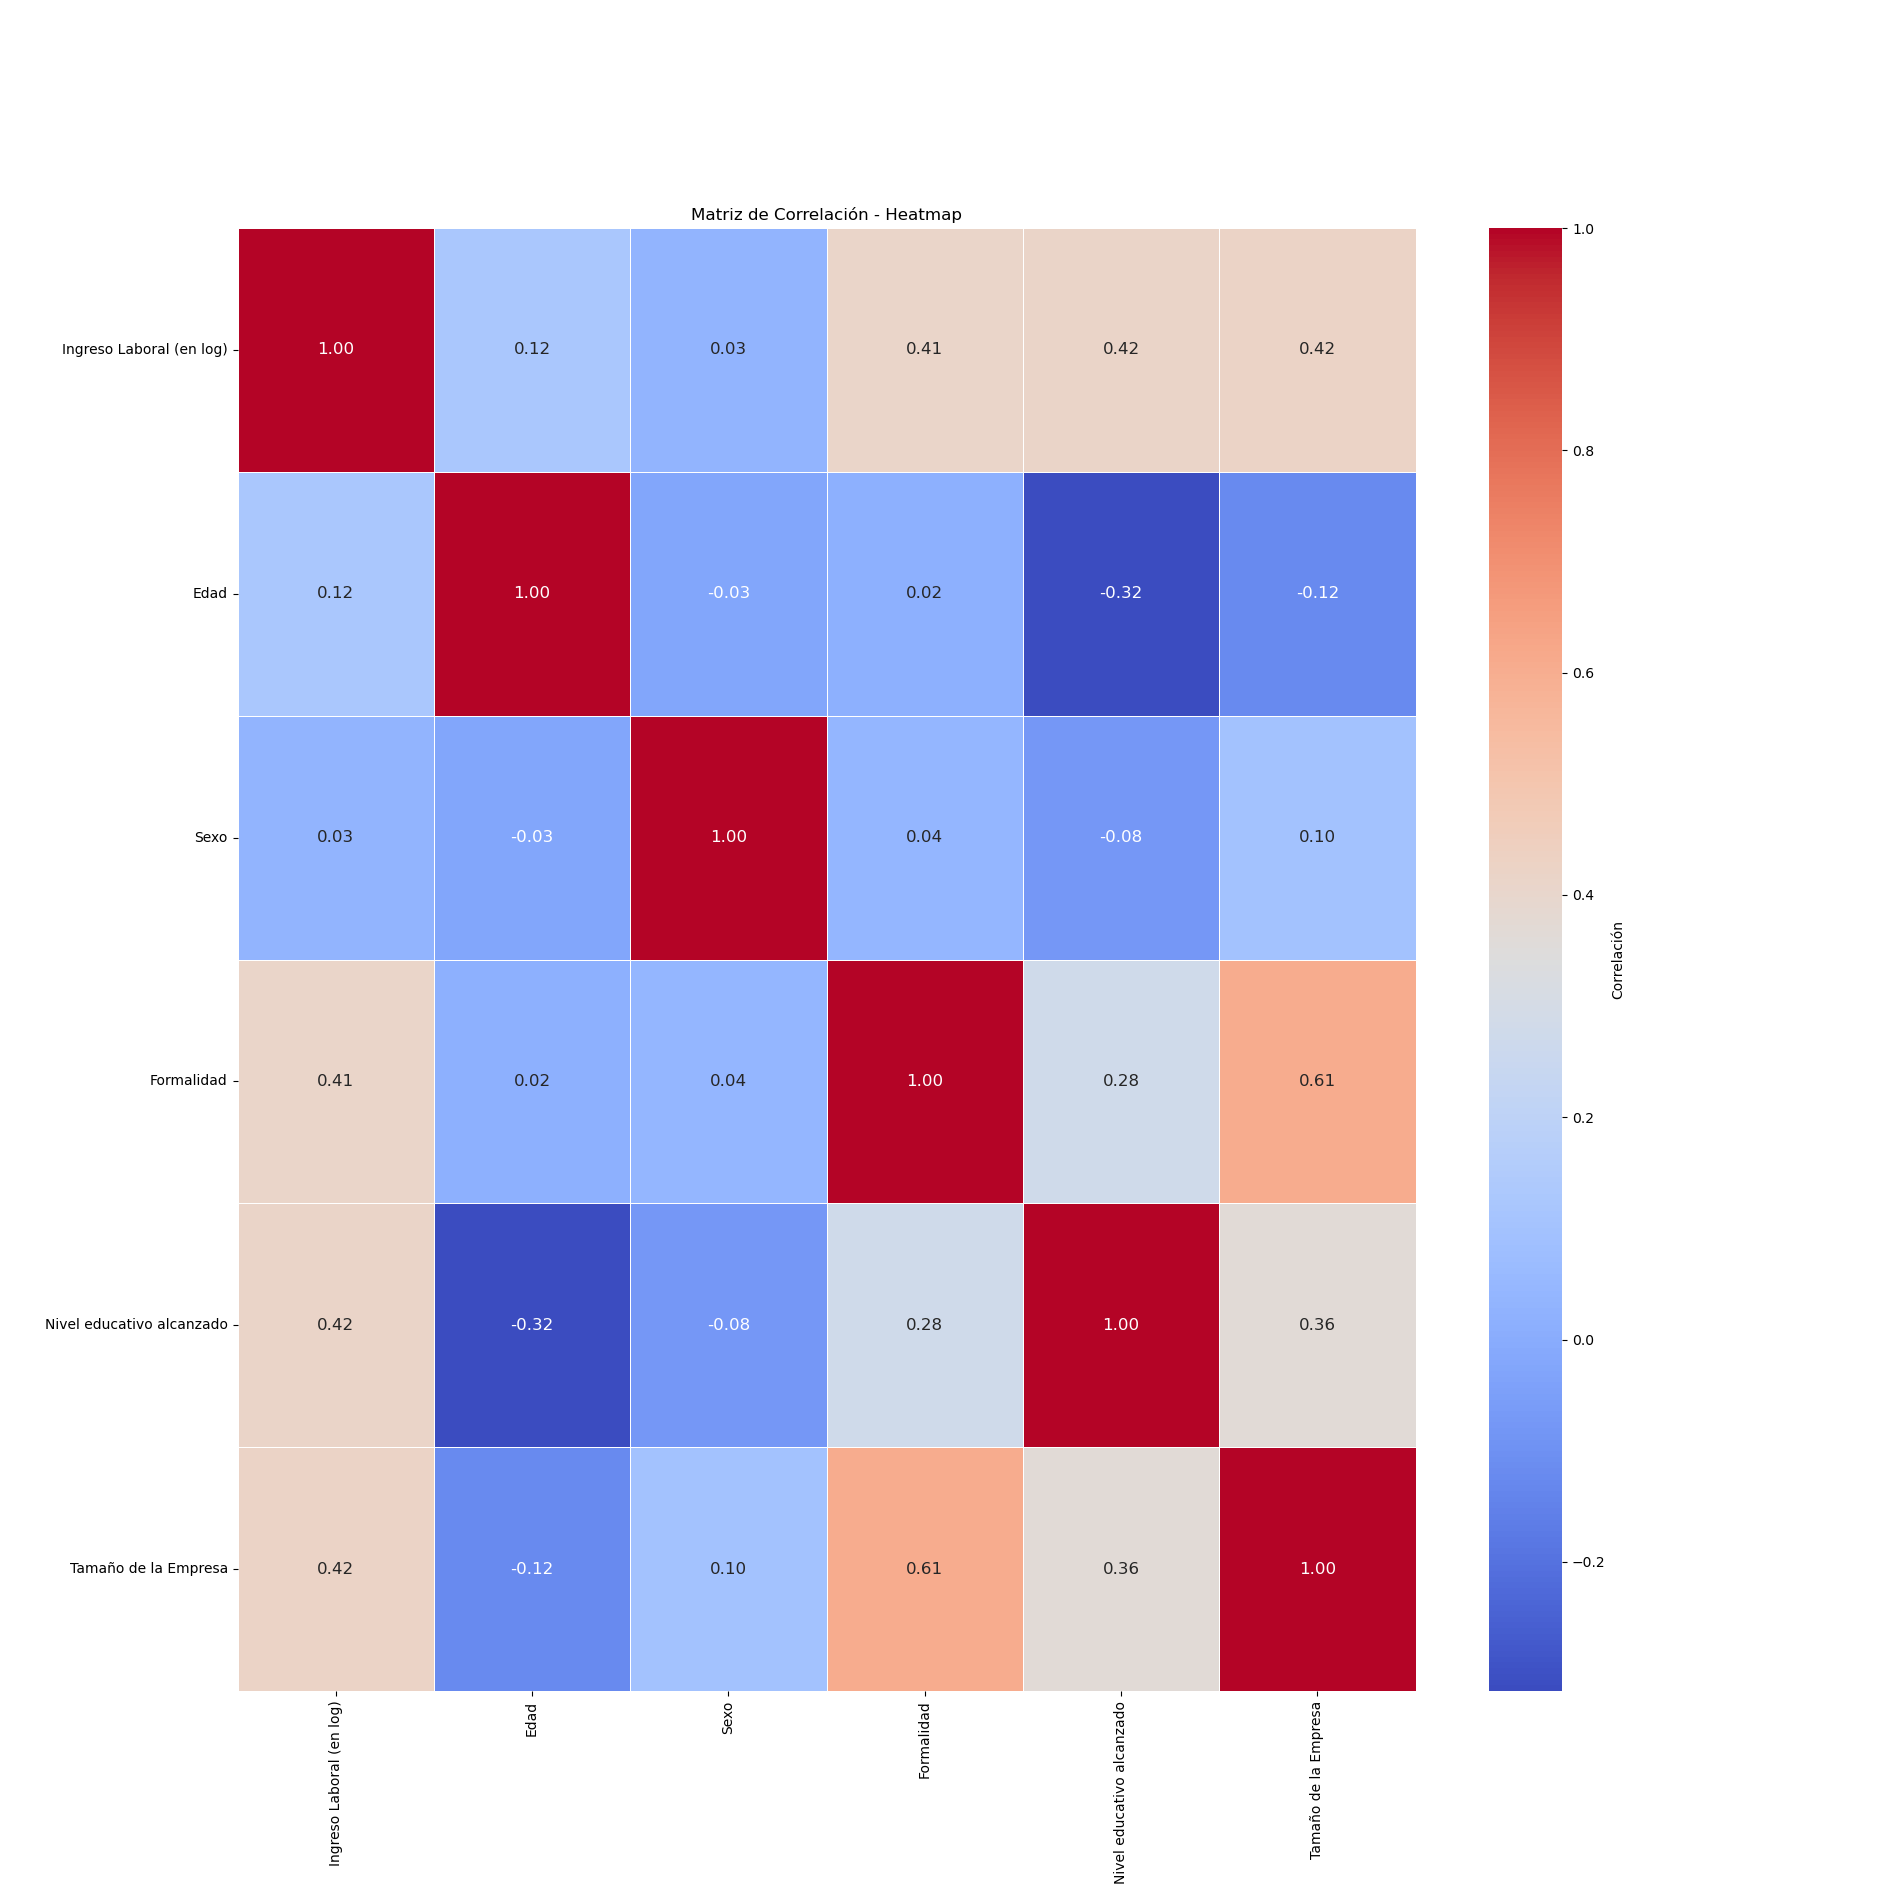
\includegraphics[width=16cm]{../Views/grafico2.png}
	\caption*{\small Fuente: Elaboración propia con base en datos de la GEIH }
\end{figure}

La matriz de correlación permite analizar las relaciones lineales entre diversas variables de interés. En este caso, se examinan las interacciones entre el logaritmo del ingreso laboral y variables como la edad, el sexo, la formalidad laboral, el nivel educativo alcanzado y el tamaño de la empresa. Destaca, en particular, la relación positiva entre el ingreso laboral y el tamaño de la empresa, el nivel educativo y la formalidad laboral, lo cual resulta coherente con las expectativas de la teoría económica. 


\section{Predicción de Salarios}

El objetivo del trabajo es construir un modelo del salario horario individual 
\begin{equation*}
w=f(X) + u  
\end{equation*}

donde \textit{w}  es el salario horario y \textit{X} es una matriz que incluye a las potenciales variable explicativas. En particular, nos centraremos es modelos lineales de la forma 
\begin{equation*}
ln(w)=\beta_0 + \beta_1 X_1 + \cdots + \beta_p X_p + u 
\end{equation*}

siendo \textit{ln(w)} el logaritmo del salario horario.


En la presente sección se analizarán una gran variedad de espeficaciones bajo el enfoque tradicional de \textit{OLS} para encontrar la mejor predicción posible del salario nominal horario de los trabajadores y comparar los resultados entre los distintos modelos especificados. 

La estimación mediante \textit{OLS} es la metodología más comúnmente empleada en economía. La misma consiste en minimizar la suma residual de cuadrados seleccionando los coeficientes $ \beta $. Esta suma residual de cuadrados es igual a la suma de los cuadrados de las diferencias entre los valores reales de la variable dependiente $y_i$ y los valores predichos por el modelo ($ \beta^{T}x_i $).  Este procedimiento permite evaluar qué tan bien se ajusta el modelo a los datos, con el objetivo de minimizar esta medida y lograr el mejor ajuste posible. Matemáticamente, el estimador de OLS se obtiene resolviendo:
\begin{equation*}
min\sum (y_i - \beta^{T}x_i)^2
\end{equation*}

Para evaluar y comparar el desempeño de las diversas alternativas modeladas se utilizarán \textit{Técnicas de Remuestreo}.  Las técnicas de remuestreo sirven para evaluar el desempeño de un modelo ya que separan los datos y los contrastan. Una parte de los datos se utiliza para entrenar al modelo, y la otra parte sirve para evaluar la precisión del mismo.  

En particular, se comenzará por utilizar la técnica de  \textit{Cross-validation}, una técnica en la que se reserva parte de los datos como conjunto de validación, mientras que el resto se utiliza como conjunto de entrenamiento. En este caso, la muestra se particionará en 70\% de entrenamiento y 30\% de prueba. 


\subsection{Modelo 1}

El primer modelo a estimar es aquel más sencillo, donde se estima al modelo sin covariables, solo una constante
\begin{equation*}
ln(w)=\beta_0 + u 
\end{equation*}

En este caso, la predicción para el logaritmo del salario laboral horario, $ \hat{y}_i $ será:
\begin{equation*}
 \hat{y}_i= \hat{\beta_1}= \frac{\sum y_i}{n}=m 
\end{equation*}

 La capacidad predictiva del modelo puede ser evaluada mediante el \textit{Mean Square Error (MSE)}, el cual asciende a 0.5405, lo cual indica que este modelo tiene escaza capacidad predictiva. La adición de covariables correlacionada con el logaritmo del salario laboral horario permitirá reducir el sesgo sin necesidad de aumentar la varianza. 

\subsection{Modelo 2}

La primer variable explicativa que se decide adicionar es la de \textit{Edad}, la cual registra los años cumplidos de cada inviduo. El modelo ya no será sólo una constante sino que contendrá una variable explicativa 
\begin{equation*}
ln(w)=\beta_0 + \beta_1 Edad + u 
\end{equation*}

Bajo esta especificación, el MSE se reduce a 0.5354 lo cual da una señal de que la edad es un buen regresor para predecir el salario laboral horario.

No obstante, la literatura empírica muestra que la relación entre la edad y en nivel de ingreso no es una relación lineal. Es más bien una relación de "U invertida" en donde los ingresos labolares al inicio de la vida de un individuo son nulos y van progresivamente aumentando durante los años activos económicamente, para luego volver a retraerse cuando se llega a la vejez.

\subsection{Modelo 3}

Una simple regresión lineal entre el logaritmo del salario y la edad no demuestra gran potencial explicativo. Como alternativa, se incluirá a continuación la edad al cuadrado para capturar esta relación no lineal.
\begin{equation*}
\ln(w) = \beta_0 +\beta_1 \textit{Edad}  + \beta_2 \textit{Edad} ^2 + u
\end{equation*}

En este nuevo modelo, el MSE continúa reduciendose a 0.5196, con lo cual la evidencia práctica demuestra la presencia de una relación no lineal entre el logaritmo del salario laboral horario y la edad, coincidiendo con los postulados teóricos. 

 \subsection{Modelo 4}

Además de la edad, el nivel educativo de un individuo, es considerado un factor clave a la hora de determinar el ingreso del trabajador, por ello se agrega como regresor a la variable \textit{maxEducLevel}. La misma registra el máximo nivel educativo alcanzado por cada individuo y consta de 7 categorías: 1. ninguno, 2. preescolar, 3. primaria incompleta, 4. primaria completa, 5. secundaria incompleta, 6. secundaria completa y 7. terciario. 
\begin{equation*}
\ln(w) = \beta_0 + \beta_1 \textit{Edad}  +\beta_2 \textit{Edad} ^2 + \beta_3 \textit{maxEducLevel}  + u
\end{equation*}

En este nuevo modelo, el MSE se reduce significativamente pasando a ser 0.3955, verificando su importancia como predictor del salario laboral. 

\subsection{Modelo 5}

Si bien en una economía igualitaria, sin brechas de género, se esperaría que la variable \textit{sexo} genere diferencias significativas a la hora de explicar el ingreso, los resultados en la matriz de correlación nos indican que dicha variable tiene una relación positiva (es decir, favorable para los hombres) con el ingreso laboral horario.  La nueva especificación del modelo tendría la siguiente forma
\begin{equation*}
\ln(w) = \beta_0 + \beta_1 \textit{Edad}  + \beta_2 \textit{Edad} ^2 + \beta_3 \textit{maxEducLevel} +\beta_4 \textit{Sexo} +  u
\end{equation*}

La adición de la variable sexo genera una reducción del MSE hasta 0.3918. Si bien constitye una mejora en el modelo de predicción, su inclusión no parece tan relevante como sí lo fue el nivel educativo. 

\subsection{Modelo 6}

Otra variable relevante para explicar al ingreso laboral horario de un trabajador es su clasificación conforme a su participación en el mercado formal o informal. En particular, se considera que un trabajador es formal si  ha realizado aportes a la seguridad social. La nueva espeficación consiste en  
\begin{equation*}
\ln(w) = \beta_0 + \beta_1 \textit{Edad}  + \beta_2 \textit{Edad} ^2 + \beta_3 \textit{maxEducLevel} +\beta_4 \textit{Sexo} +\beta_5 \textit{Formal}  + u
\end{equation*}

El MSE se reduce hasta 0.3556, lo cual verifica que la pertenencia a un grupo u otro de trabajadores es relevante en la determinación de los salarios que perciben los trabajadores. 

\subsection{Modelo 7}

Además del sector en el que se encuentra empleado un trabajador (formal o informal), el tamaño de la empresa en la cual ofrecen su empleo puede ser determinante del salario que percibe. En la matriz de correlación se observó que el tamaño de la empresa tenía una relación positiva con el ingreso labora, esto es, aquellas empresas con mayor cantidad de empleados reportaban mayores ingresos. 

La variable de interés para incluir a nuestro modelo es la denomina en la muestra \textit{sizeFirm}, la cual adopta 5 valores: 1. autónomo, 2.  2-5 empleados, 3. 6 -10 empleados, 4. 11-50 empleados y 5. más de 50 empleados

El nuevo modelo a estimar es 
\begin{equation*}
\ln(w) = \beta_0 + \beta_1 \textit{Edad}  + \beta_2 \textit{Edad} ^2 + \beta_3 \textit{maxEducLevel} +\beta_4 \textit{Sexo} +\beta_5 \textit{Formal}  + \beta_6 \textit{SizeFirm} +  u
\end{equation*}

El nuevo regresor contribuye a la predicción del salario laboral, alcanzando un MSE de 0.3420.

\subsection{Modelo 8}

Además de los regresores incluídos hasta el momento, otra variable potencialmente relevante en el predicción del salario es el tipo de relación familiar del hogar. En particular, se esperaría que el jefe de hogar cuente con un salario superior al del resto de miembros del hogar, dado su carácter de jefe y proveedor. A tal fin, se crea, a partir de la variable \textit{P6050} contenida en la muestra la cual indica cual es el parentesco con el jefe de hogar,  una variable dummy que toma valor 1 en cado de que el individuo reporte ser jefe del hogar y 0 en caso contrario.  De esta manera la nueva especificación consite en 
 \begin{equation*}
\ln(w) = \beta_0 + \beta_1 \textit{Edad}  + \beta_2 \textit{Edad} ^2 + \beta_3 \textit{maxEducLevel} +\beta_4 \textit{Sexo} +\beta_5 \textit{Formal}  + \beta_6 \textit{SizeFirm} + \beta_7 \textit{Jefe} +  u
\end{equation*}

A diferencia de todas las especificaciones anteriores, esta es la primera oportunidad donde el MSE no se ve alterado permaneciendo en 0.3420. Ello indica que la inclusión de este nuevo regresor no permitió reducir el sesgo sin adicionar mayor varianza. Es posible que la variable jefe no sea estadísticamente relevante o que nos estemos acercando a un punto de sobreparametrización del modelo, donde el sesgo no se reduce pero la varianza aumenta. 

\subsection{Modelo 9}

La literatura dedicada a la economía laboral postula que un mayor ingreso no laboral atenta contra la oferta de trabajo tanto en margen extensivo como en margen intensivo. Para testear si el ingreso no laboral es una variable relevante en la explicación del salario, se incorpora una dummy que vale 1 cuando el individuo percibe algún tipo de ayuda estatal. Para la construcción de dicha variable se utilizaron diversas variables disponibles en la muestra que hacen referencia a la percepción de subsidios por parte del individuo (\textit{P6858s1, P6858s2, P6858s3 y P6858s4}).  El modelo a estimar es
\begin{equation*}
\begin{aligned}
\ln(w) = &\ \beta_0 + \beta_1 \textit{Edad} + \beta_2 \textit{Edad}^2 + \beta_3 \textit{maxEducLevel} 
         + \beta_4 \textit{Sexo} + \beta_5 \textit{Formal} + \beta_6 \textit{SizeFirm} \\
         &+ \beta_7 \textit{Jefe} + \beta_8 \textit{Subsidio} + u
\end{aligned}
\end{equation*}

La predicción del modelo mejora sustancialmente con un MSE de 0.2887. De esta manera, se observa que todavía no nos encontramos en un escenario de sobreparametrización, sino que existe un margen para continuar mejorando el sesgo. 


\subsection{Modelo 10}

Finalmente, se parte del último modelo estimado y se adicionan la interacción de ciertas variables incluídas hasta entonces: \textit{maxEducLevel $\times$ Sexo} y \textit{Formal $\times$ Sexo}.  El modelo a estimar resulta en 
\begin{equation*}
\begin{aligned}
\ln(w) = &\ \beta_0 + \beta_1 \textit{Edad} + \beta_2 \textit{Edad}^2 + \beta_3 \textit{maxEducLevel} 
         + \beta_4 \textit{Sexo} + \beta_5 \textit{Formal} + \beta_6 \textit{SizeFirm} \\
         &+ \beta_7 \textit{Jefe} + \beta_8 \textit{Subsidio} + \beta_9 \textit{(maxEducLevel $\times$ Sexo)} 
         + \beta_{10} \textit{(Formal $\times$ Sexo)} + u
\end{aligned}
\end{equation*}

Con esta última especificación es donde obtenemos la mejor predicción del modelo con un MSE de \textbf{0.2877}.

Si bien la adición sucesiva de regresores, conformados por distintas variables explicativas como de distintas no linealidades de las mismas, permitieron construir un modelo para el logaritmo del salario laboral horario cada vez más eficiente, ello no sucede si se incorporar nuevos regresores que no sean significativos para predecir al salario, en particular se alcanzaría un punto donde el MSE comenzaría a aumentar nuevamente. La reducción del sesgo tras incorporar nuevas variables explicativas no alcanzaría a compensar el incremento en la varianza ocasionada por dicha inclusión. 

A su vez, la técnica utilizada hasta entonces para evaluar el desempeño de los distintos modelos (\textit{Validation Set Approach}) es bastante útil presenta dos debilidades principales:  El primero es que, dado un conjunto de datos original, si se reserva una parte para probar el modelo, queda menos información disponible para la estimación (lo que reduce la eficiencia), el segundo problema radica en decidir qué datos se utilizarán para entrenar el modelo y cuáles para probarlo.

\subsection{Análisis de los errores}
Dado que el modelo 10 registra el menor error cuadrático (MSE) medio entre todos los modelos propuestos, pero aún así su MSE no es cero, resulta de interés ver la dispersión de estos errores. Además, se destacan aquellos errores debido a \textit{outliers} en las observaciones.

La figura 3 muestra la dispersión de los errores de las predicciones realizadas sobre el conjunto de prueba. Un modelo con una buena estimación tiene la mayor cantidad de observaciones posibles alrededor del cero. Se observa que muchos de los errores de estimación están efectivamente alrededor del cero, mientras que hay algunos errores que presentan mayor dispersión. 

Dado que los errores más alejados del cero no siguen un patrón determinado y su distribución parece aleatoria, se podría sugerir que no hay fallas sistemáticas en el modelo estimado y aquellos individuos alejados de la muestra podrían resultar de interés para una agencia de recaudación como la Dirección de Impuestos y Aduanas Nacionales (DIAN).
\begin{figure}[H]
    \centering
	\caption*{\textbf{Figura 3. Dispersión de los errores de predicción, modelo 10.}}
	\captionsetup{justification=centering}
	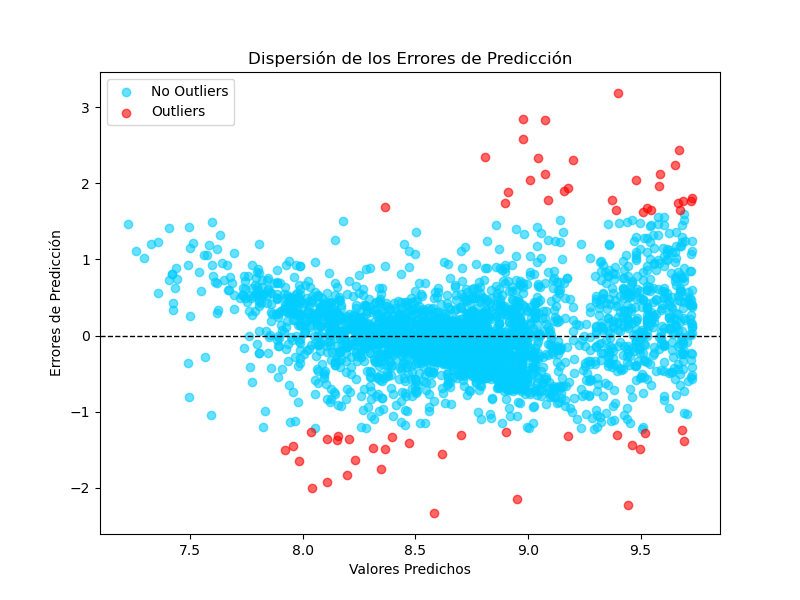
\includegraphics[width=16cm]{../Views/grafico4.png}
	\caption*{\small Fuente: Elaboración propia con base en datos de la GEIH }
\end{figure}

\subsection{Leave-one-out cross-validation (LOOCV)}
Como técnica de remuestreo superadora se utilizará \textbf{\textit{Leave-one-out cross-validation (LOOCV)}}. A diferencia de la técnica anterior,  el modelo se entrena con todas las observaciones excepto una, y luego se evalúa con la observación excluida. Es decir, cada muestra en los datos se utiliza una vez como conjunto de validación, y el modelo se entrena con las muestras restantes. 

La estimación de LOOCV para el error cuadrático medio (MSE) de prueba es:
\begin{equation*}
\text{LOOCV}(n) = \frac{1}{n} \sum \text{MSE}_{-i} 
= \frac{1}{n} \sum (y_i - \hat{y}_{-i})^2
\end{equation*}
donde $-i$ indica que el modelo para obtener la predicción fue entrenado con todas las observaciones excepto en la observación $i$.

A pesar de que LOOCV es computacionalmente costoso, es más exhaustivo en la evaluación del modelo, ya que cada muestra se utiliza como conjunto de validación exactamente una vez, proporcionando una evaluación más completa del desempeño del modelo. 


\section{Conclusiones}
El presente análisis ha permitido explorar distintos modelos de predicción para el salario laboral horario de los trabajadores en Colombia, utilizando datos de la Gran Encuesta Integrada de Hogares (GEIH) de 2018. 

Se analizaron diversas especificaciones lineales para predecir el salario laboral horario adicionando sucesivamente variables explicativas tales como la edad, el sexo, el nivel educativo máximo alcanzado por los hogares, la pertenencia al sector formal entre otros, como así también distintas especificaciones de las mismas, como la edad al cuadrado o las interacciones entre nivel educativo y sexo o sexo y formalidad. 

La Tabla 2 resume el error cuadrático medio obtenido en las distintas espeficaciones y utilidando dos estrategias de remuestro: \textit{Validation Set Approach} y textit{Leave-one-out cross-validation (LOOCV)}.

\begin{table}[ht]
    \centering
    \caption*{\textbf{Tabla 2. MSE de los Modelos}}
    \begin{tabular}{lcc}
        \toprule
        \textbf{Modelo} & \textbf{MSE} \\
        \midrule
        \textbf{Validation Set Approach} & \\
        Modelo 1 & 0.540521 \\
        Modelo 2 & 0.535473 \\
        Modelo 3 & 0.519642 \\
        Modelo 4 & 0.395526 \\
        Modelo 5 & 0.391781 \\
        Modelo 6 & 0.355572 \\
        Modelo 7 & 0.341998 \\
        Modelo 8 & 0.341998 \\
        Modelo 9 & 0.288723 \\
        Modelo 10 & 0.287787 \\
        \midrule
        \textbf{LOOCV} & \\
        Modelo 9 & 0.540380 \\
        Modelo 10 & 0.540380 \\
        \bottomrule
    \end{tabular}
\end{table}


De la misma se concluye que la adición de variables fue exitosa en la mejora de la predicción de los salarios, no obstante se esperaría que de continuar con la adición de variables se conduzca a una sobreparametrización donde el incremento de la varianza por la inclusión de nuevas variables sea superior a la reducción del sesgo. 

Asimismo, se observa que con la técnica de LOOCV, la capacidad predictiva de los dos mejores modelos (modelo 9 y 10) analizado bajo la técnica de remuestro anterior se ve sumamente reducida.


\end{document}
